% Welcome, Math for Math's sake folks!
%
% My idea is to use this file as a way to share solutions, questions, and comments.
%
% Feel free to edit any part of it, and add ``Your name:your comment, question, or solution'' so we know who is asking what.
%
% You don't have to worry too much about making mistakes in LaTeX format: ShareLatex keeps track of the file's history, so it's pretty easy to fix mistakes.  There's help here if you want to learn LaTeX and ShareLatex: https://www.sharelatex.com/learn
%
% If you're a techy person, this is also linked to a github repo here: https://github.com/mkoconnor/Topology-Chapter-2 Feel free to submit a pull request.  If you've never heard of github, just ignore this paragraph.
%
% This is a total experiment, and I'm not sure if will people will like or use it, but let's find out!
\documentclass{article}
\usepackage[utf8]{inputenc}
\usepackage{amssymb, amsmath}
\usepackage{mathabx}
\usepackage{tikz}
\usetikzlibrary{automata,positioning}

\title{Topology, Chapter 2}
\author{Math for Math's Sake}
\newcommand\s{\section*}
\renewcommand\ss{\subsection*}
\newcommand\sss{\subsubsection*}
\newcommand\ms{Michael's solution: } % easy way to mark my solutions
\newcommand\mt{Michael's thought: } % easy way to mark my thoughts
\newcommand\pf{Peter's solution: } % Same for mine

\begin{document}
\maketitle
\s{13}
\ss{13.1}
For each $x$, let $U_x$ be an open set containing $x$ and inside $A$.  Then $A =
\bigcup_{x\in A}U_x$, which is open, since it's a union of open sets.
\ss{Find all topologies on $\{a,b\}$ and decide which are finer than which}
This diagram shows all four topologies with the finer topologies higher up.
\begin{center}
  \tikzstyle{every node}=[rectangle]
  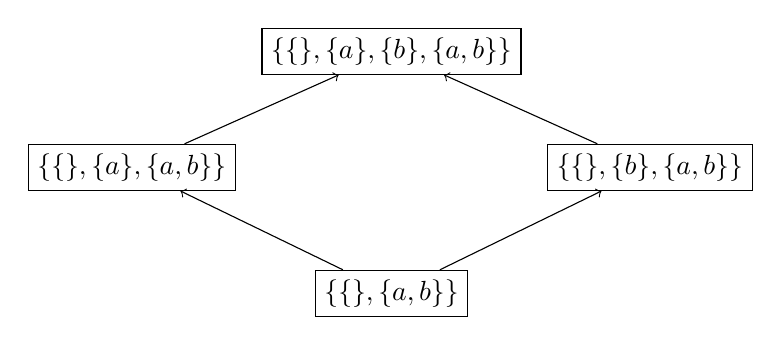
\begin{tikzpicture}
    \node (empty) [draw] {$\{\{\},\{a,b\}\}$};
    \node (a) [draw,above left=of empty] {$\{\{\},\{a\},\{a,b\}\}$};
    \node (b) [draw,above right=of empty]   {$\{\{\},\{b\},\{a,b\}\}$};
    \node (phantom) [above=of empty] {$\phantom{0}$};
    \node (all) [draw,above=of phantom] {$\{\{\},\{a\},\{b\},\{a,b\}\}$};
    \path[->] (empty) edge (a);
    \path[->] (empty) edge (b);
    \path[->] (a) edge (all);
    \path[->] (b) edge (all);
  \end{tikzpicture}
\end{center}
\ss{13.3}
We have that $\mathcal{T}_c$ is a topology as it contains both $\{\}$ and $X$ and, if $S$ is a collection of sets such that $X-U$ is countable for every $U\in S$, then the same must be true for $\bigcup S$, since $U\subseteq\bigcup S$ for every $U\in S$.  Similarly for intersections.

On the other hand, $\mathcal{T}_\infty$ is not a topology.  Let $X=\mathbb{N}$; then $\{2n\}\in\mathcal{T}_\infty$ for all $n\in\mathbb{N}$, but the union of all those sets isn't.

{\it Adam's re-phrased proof}:  Of course $\{\}, X$ are both in $\mathcal{T}_c$ by an easy direct verification.  Let $U_\alpha$ be some indexed collection of sets in $T_c$ which by definition implies $X-U_\alpha$ is either $X$ or countable.  We want to show that $\bigcup U_\alpha\in \mathcal{T}_c$ which also means showing that $X-\bigcup U_\alpha$ is either $X$ or countable.  If at least one $U_a$ is not empty then $X-U_a$ is countable and $X-\bigcup U_\alpha \subseteq X-U_a$ and so $X-\bigcup U_\alpha$ is countable hence $\bigcup U_\alpha\in \mathcal{T}_c$ as desired.  

The proof for intersections goes similarly.  

\ss{13.4}
\sss{13.4(a)}
$\bigcap\mathcal{T}_\alpha$ is a topology as it contains the empty set and $X$, and if some family of sets $\{U_i\}$ is a subset of $\bigcap\mathcal{T}_\alpha$, it must be a subset of each $\mathcal{T}_\alpha$.  Thus, $\bigcup\{U_i\}$ must be in each $\mathcal{T}_\alpha$, and therefore it must be in $\bigcap\mathcal{T}_\alpha$.  Similarly for intersections.

On the other hand, $\bigcup\mathcal{T}_\alpha$ need not be a topology: Consider $X=\{a,b,c\}$, $\mathcal{T}_1 = \{\{\},\{a\},\{a,b,c\}\}$ and $\mathcal{T}_2=\{\{\},\{b\},\{a,b,c\}\}$.
\sss{13.4(b)}
The unique smallest topology containing each $\mathcal{T}_\alpha$ can be found by taking the intersection of all topologies containing each $\mathcal{T}_\alpha$ (which we know is a topology by part a).

The unique largest topology contained in each $\mathcal{T}_\alpha$ is $\bigcap\mathcal{T}_\alpha$.
\ss{13.5}
The intersection of all topologies on $X$ containing $\mathcal{A}$ must be a subset of the topology generated by $\mathcal{A}$, since the topology generated by $\mathcal{A}$ \textit{is} one of the topologies being intersected.

On the other hand, every topology containing $\mathcal{A}$ must contain everything in the topology generated by $\mathcal{A}$, since they must all be closed under unions, finite intersections, and contain the empty set and the whole space.
\s{16}
\ss{16.1} {\it Adam:} Let's call the topology $A$ inherits as a subspace of $X$ the topology $\mathcal{T}_X$ and call $\mathcal{T}_Y$ likewise, and we want to show $\mathcal{T}_X=\mathcal{T}_Y$.  Begin by taking any open set $U\in \mathcal{T}_X$ and let us see why $U\in \mathcal{T}_Y$.  From the assumption that $U\in \mathcal{T}_X$ we know there is a $O\in \mathcal{T}$ (the topology on $X$) such that $U=A\cap O$.  In order to show what we want, we must find an $\tilde{O}$ open in $Y$ such that $U = A\cap \tilde{O}$, but then being open in $Y$ means that there is some $V\in \mathcal{T}$ such that $\tilde{O}=Y\cap V$.  So our goal reduces to finding some $V\in \mathcal{T}$ such that $U=A\cap (Y\cap V)$. Of course $O$ is the correct choice for $V$ the proof of which I leave to the reader---but the main relevant observation is that $A\subseteq Y$.

The other direction should go similarly.
\ss{16.2} {\it Adam:} The subspace induced by $\mathcal{T}'$ is finer but not necessarily strictly finer than that induced by $\mathcal{T}$.
\ss{16.3} {\it Adam:} $A,B,E$
\ss{16.8} {\it Adam:} $\mathbb{R}_\ell\times \mathbb{R}$ basically permits lower-limits on the $x$-axis but not on the $y$ ... but you need both to get the lower-left point if that segment of the line were going to be permitted (assuming $L$ does not run horizontally in which case the topology would just be the lower-limit topology).  Hence this is just the usual topology on a line.  But for $\mathbb{R}_\ell\times \mathbb{R}_\ell$ we get lower-limits in both axes and so whether the line is horizontal or not we get the lower-limit topology on the line.  
\s{17}
\ss{17.1} {\it Adam}: The proof here goes almost identically the way that 13.3 did.
\ss{17.2} {\it Adam:} I'll assume that the topology for the whole space, $\mathcal{T}$, is on $X$, which I don't have to do but it will make things easier and I think it still performs the intended exercise.  

We want to show that $X-A\in \mathcal{T}$ from the facts that $X-Y\in \mathcal{T}$ and that $A$ is closed in $Y$.  That $A$ is closed in $Y$ is for the subspace topology, so that by saying $Y-A$ is in this topology means that there is some open set $O\in \mathcal{T}$ such that $Y\cap O=Y-A$.  Unless someone sees a better way of going about this, probably we want to show $X-A\in \mathcal{T}$ by showing that it is a union or intersection of other sets that we know are open, somehow.  If you play with Venn diagrams long enough using $X,Y,$ and $A$ you'll probably realize first that $A\subseteq Y\subseteq X$ just because of one thing being in another space easily implies this, and also $X-A=X-Y\cup Y-A$.  It should at this point be easy to show (perhaps by reference to a theorem in section 16) that $Y-A$ is open in $\mathcal{T}$ and therefore $X-A$ is open in $\mathcal{T}$.  
\ss{17.5} {\it Adam}: Since $\overline{(a,b)} = (a,b)\cup (a,b)'$ and $(a,b)\subseteq [a,b]$ then all that remains is to show that $(a,b)'\subseteq [a,b]$.  This amounts to showing that, if $x<a$ then $x$ is not a limit point, and likewise for $b$.  But then $x\in (-\infty,a)$ so the result holds.  

Equality holds if the space has the least upper bound property or maybe it's density ... I'll let you guys teach me this one.
\ss{17.6 (a)} {\it Adam:} The most significant portion of this is showing $A'\subseteq \overline{B}$, so letting $x\in A'$ and $x\in U\in \mathcal{T}$ then there is some $x\ne y\in U\cap A\subseteq U\cap B$.  Hence $x\in B'\subseteq \overline{B}$.
\ss{17.6 (b)} {\it Adam:} I'll do the $\Rightarrow$ direction and assume the reverse isn't much harder.  If $x\in \overline{A\cup B}$ and $x\in U\in \mathcal{T}$ let's assume $U\cap A=\{\}$ and show $U\cap B\ne \{\}$.  If you understand the motivation for this setup, it's actually practically trivial to show $U\cap B\ne \{\}$ from the assumptions so far.
\ss{17.6 (c)} {\it Adam:} This proof should mimic the $\Leftarrow$ proof you give to part (b).  A counter-example is $A_{n} = [1-1/n,2-1/n]$ for $n\in \mathbb{Z}^+$.
\ss{17.7}  $x$ will not necessarily be a limit point of $A_\alpha$ because of the method by which the neighborhood and $A_\alpha$ were selected to be associated.  It is illegitimate to first pick the neighborhood $U$ and then find a set intersecting it---you must argue that $x$ is a limit point of a given $A_\alpha$ by specifying $A_\alpha$ first and then for this fixed set, show that any neighborhood around $x$ will intersect it.
\ss{17.10} {\it Adam:} Supposing $x_1<x_2$ then $U_1 = (-\infty, x_2),U_2=(x_1,\infty)$.
\ss{17.14} {\it Adam:} For spaces $(X,\mathcal{S})$ and $(Y,\mathcal{T})$, if $(x_0^0,x_0^1)\ne (x_1^0,x_1^1)\in X\times Y$ and $U_{i,j}$ for $i,j=0,1$ disjointly covers $x_i^j$, then call $A=U_{0,0}\times U_{0,1}$ and $B=U_{1,0}\times U_{1,1}$, then I'm pretty sure $A$ covers precisely the first point, and $B$ covers precisely the second.  I'm being sloppy for time and to let you fill in the details yourself.
\ss{17.15} {\it Adam:} For the $\Rightarrow$ direction suppose the $T_1$ condition holds for some space and let $x_1\ne x_2$.  Then $\{x_1\}$ is closed so $X-\{x_1\}$ is a neighborhood of $x_2$ not containing $x_1$ and the other neighborhood is similar.  The converse should be just as simple.
\ss{17.19}
\end{document}
